\documentclass[12pt,fleqn]{article}
\setlength{\parindent}{0pt}
\usepackage{graphicx}
\usepackage{listings}
\usepackage[latin5]{inputenc}
\setlength{\parskip}{8pt}
\setlength{\parsep}{0pt}
\setlength{\headsep}{0pt}
\setlength{\topskip}{0pt}
\setlength{\topmargin}{0pt}
\setlength{\topsep}{0pt}
\setlength{\partopsep}{0pt}
\setlength{\mathindent}{0cm}

\begin{document}
MIT OCW Cok Degiskenli Calculus - Ders 6

Bir onceki derste cycloid konusunu isledik. 

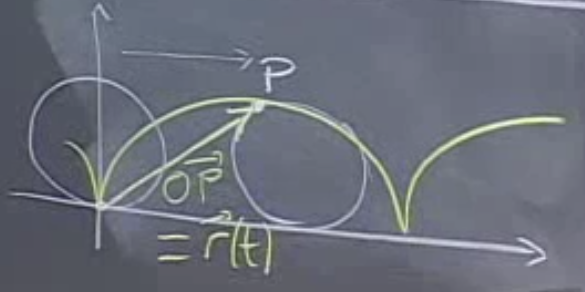
\includegraphics[height=4cm]{6_1.png}

Hareket eden bir noktanin pozisyonu

\[ (x(t), y(t), z(t)) \]

Bu noktayi takip etmenin diger yollarindan biri onu pozisyonu vektoru
olarak gormek, ki bu vektorun bilesenleri noktanin kordinatlari. 

\[ \vec{r}(t) = <x(t),y(t),z(t)> \]

Vektor orijin (baslangic) noktasindan gelinen noktayi isaret eden bir
vektor (resimde $\vec{OP}$). 

Cycloid probleminde tekerlek yaricapini 1 alalim ve birim hizda ilerliyor
olalim, ki boylece aci $\theta$ ve zaman ayni sey haline gelsin

\[ \vec{r}(t) = <t-sin(t), 1-cos(t) \]

Tamam. Simdi, noktanin pozisyonunu zaman acisindan bildigimize gore, onun
degisimini inceleyebiliriz, mesela hizina, ivmesine bakabiliriz. Ilk once
hiza bakabiliriz. Fakat, aslinda, hizdan daha iyisini hesaplayabiliriz. Hiz
tek bir sayidir sadece, ama eger su icinde GPS olan satafatli spor
arabalarindan birine sahip degilseniz, size hizinizin ``hangi yonde''
oldugunu soylemez. Sadece ``gittiginiz yonde'' (her ne yone gidiyorsaniz)
ne kadar hizli oldugunuzu soyler.

O zaman biz hizimizi hesaplarken, hem yonu, hem hizi ayni anda goze
alabiliriz. Bu demektir ki vektor kavrami tekrar isimize yarayacak. Hizi
vektor olarak hesaplayabiliriz. 

Bunu nasil yapariz? Pozisyon vektorunun zamana gore turevini alabiliriz.

\[ \vec{v} = \frac{d\vec{r}}{dt} \]

Bu tur bir turevi bu derste ilk kez goruyoruz, ilk kez bir vektorun
turevini aliyoruz. Bu sekilde turev almak demek, o vektorun bilesenlerinin
teker teker turevini almak demektir. Yani

\[ =
<\frac{dx}{dt}, \frac{dy}{dt}, \frac{dz}{dt}>
\]


Cycloid ornegine donersek

\[ \vec{r}(t) = <t-sin(t), 1-cos(t) \]

formulunun turevini alirsak ne olur? 

\[ \vec{v} = \frac{d\vec{r}}{dt} = <1-cos(t),sin(t)>\]

Iste bu turev bize hangi yonde ve ne kadar hizli gittigimizi gosteriyor. 

Bu arada bir vektorunun buyuklugunun (magnitude) her zaman mesafesel,
uzakliksal anlami olmayabilecegini de gormus oluyoruz. Hiz kavrami bir
orandir, katedilmis bir mesafe, bir yer degildir, $t$ aninda bir yonde olan
bir buyukluktur. Fakat yine de bir buyukluktur, bir yonu vardir, ve bu
sebeple vektorler ile temsil edilebilir. 

Problemimize donelim. Onceki derste tekerlekte izlenen noktanin en alta gelip
yukseldigi siralarda hareketinin nasil oldugunu irdelemistik. Simdi bu
konuyu hiz kavramini kullanarak incelemeye ugrasalim. Ustteki vektore $t=0$
koyarsam, ne olur? Sonuc $<0,0>$, yani $\vec{v} = 0$. Tabii ki nokta $t=0$
oncesi hareket ediyor, sonra da ediyor, yani bir hizi var, sadece ``o
anda'' hizi yok. 

Peki hiz vektor olarak daha fazla bilgi veriyor olmasina ragmen, ben yine
de klasik anlamda hizi, yani o tek sayiyi elde etmek istiyorsam ne yaparim?
Hiz vektorunun buyuklugunu hesaplarim, $|\vec{v}|$. 

\[ |\vec{v}| = \sqrt{ (1-cos(t))^2 + sin^2(t) } \]


\[ = \sqrt{ 1-2cos(t) + cos^2(t) + sin^2(t)  } \]


\[ = \sqrt{ 2-2cos(t) } \]


Bu formule bakarak hizin nerede en fazla, en az oldugunu
hesaplayabiliriz. Eger $t=0$ ise, sonuc sifir olur. $t=\pi$ ise elimizde
$\sqrt{4} = 2$ vardir, bu an noktanin tekerlegin en ustunde oldugu andir,
bu an ayni zamanda en hizli hareket ettigimiz de andir. Hatta bu hiz
tekerlegin saga dogru yatay gidis hizinin iki katidir, tekerlegin saga
dogru birim hizda ilerledigini soylemistik, fakat nokta bunun ustune bir de
merkeze gore bir donme hareketi icinde, ve bu iki etki birbirine eklenerek
$2$ hizina sebebiyet veriyor.

O nokta tepe noktasindan asagi inmeye baslayinca tabii ki noktamiz donusun
``geriye dogru'' olan etkisiyle toplami hizinda dusme yasiyor.

Ivme

Bu konuyu islemeden once klasik olarak bilinen ivme kavrami ile burada
kullanacagimiz ivme kavrami ile ciddi uyusmazliklar oldugunu
belirtmeliyim. Klasik anlayista ivme mesela bir arabada giderken
``hissettigimiz sey'' bizi koltuga iten kuvvet, hizdaki degisim (hizin
turevi) olarak bilinir, ve eger bir arabada saatte 40 km ile gidiyorsam,
ivme yok denir. Fakat simdi bu arabanin bir virajdan dondugunu farzedelim,
bu durumda bir kuvvet hissederiz, hala saatte 40 ile gidiyor olabilirim,
ama bir ivme vardir. Burada aslinda yana dogru bir hizlanma / ivme
sozkonusudur. O zaman yine vektor kavramini kullanmamiz lazim. 

Ivme vektorunu soyle belirtelim:

\[ \vec{a} = \frac{d\vec{v}}{dt} \]

Fizikteki ivme tanimi da budur, $F = ma$ derken kastedilen $a$ iste bu
$a$'dir. Bir vektordur. 

Cycloid'e donelim. 

\[ \vec{v} = <1-cos(t),sin(t)>\]

Turevi alalim

\[ \frac{d\vec{v}}{dt} = <sin(t), cos(t)>\]

$t=0$ noktasinda ivme nedir? $<0,1>$. 

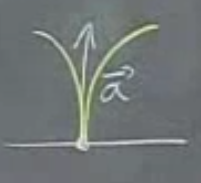
\includegraphics[height=3cm]{6_2.png}

Yani $t=0$ anindaki ivme bir birim vektor, ve yonu tam yukariya dogru. Bu
ilginc bir sey, o anda hiz sifir, fakat bir ivme mevcut. 

Bu arada, hemen belirtelim

\[ \bigg|\frac{d\vec{r}}{dt}\bigg|  \ne \frac{d|\vec{r}|}{dt}\]


Yani bir vektorun turevinin buyuklugu, o vektorun buyuklugunun turevi ile
ayni sey degildir. Esitsizligin sagindaki kavram zaten cogunlukla pek ise
yarar bir sey degildir, hesaplanabilir, biraz sac bas yoldurabilir ama
mumkundur, fakat cogunlukla kullanilmaz. 

Egri Uzunlugu (Arc Length)

Egri uzunlugu bir egri uzerinde ne kadar yol katettigimizi gosteren bir
buyukluktur. Mesela bir arabadaki ne kadar yol katettiginizi gosteren
kilometre sayaci bunu arabanin hizini belli bir zaman uzerinden entegre
ederek hesapliyor.

$s$ = bir yol uzerinde katedilmis mesafe

Bunun anlami olmasi icin tabii ki bir sabit, referans noktasi
dusunmeliyiz. Orijin noktasi bu nokta olabilir. Bu arada $s$ referans
noktasinin neresinde oldugumuza gore negatif olarak ta
hesaplanabilir. Referansa kadar eksi, sonrasi arti olabilir mesela.

Peki $s$ ile $t$, yani egri uzunlugu ve zamani nasil birbirine baglariz? 

\[ \frac{ds}{dt} = \textrm{ h�z } = |\vec{v}| \]

Yani birim zamanda katedilen egri uzunlugu hizdir. 

Ama acik olmak gerekirse, aslinda turevin kesin degerini (absolute value)
almak daha dogru olur (dikkat, vektor buyuklugu isareti degil, kesin deger
isareti bu sefer)

\[ \bigg| \frac{ds}{dt} \bigg| = \textrm{ h�z } = |\vec{v}| \]

Niye? Belki bir egri uzerindeyiz ama o egri uzerindeki hareketimiz bir
ileri bir geri seklinde. Bu durumda egri uzunlugunu surekli saymak
istemeyiz, onu ``cogalan (ileri), azalan (geri)'' turunden bir buyukluk
olarak gormek isteriz.

Egri uzunlugu hesabi icin hizi zaman uzerinden entegre ederiz. Mesela bir
cycloid'in (resimde sari ile gosterilen) bir turunun uzunlugu ne kadar diye
hesaplamak istiyorsak, 

\[ \vec{v} = \sqrt{ 2-2cos(t) } \]

ifadesinin 0 ile $2\pi$ arasinda entegralini almamiz lazim. 


\[ \int_o^{2\pi} \vec{v} = \int_o^{2\pi} \sqrt{ 2-2cos(t) } dt \]

Acikca soylemek gerekirse bunun entegrali analitik olarak nedir bilmiyoruz,
ama ileriki derslerde bu hesabi yapmak icin fiyakali bir numara gorecegiz. 

Gidisatin Birim Teget Vektoru

Notasyonda bu kavram cogunlukla $\hat{T}$ olarak gosterilir. Sapka var
cunku vektor birim vektor. $T$ cunku ``teget''. 

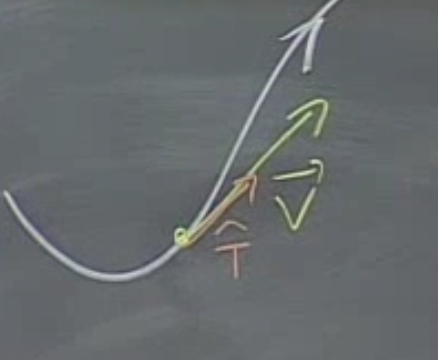
\includegraphics[height=2cm]{6_3.png}

Vektor $\vec{v}$ gidisata (trajectory) zaten tegettir (dikkat, bu illa
pozisyon vektoru $\vec{r}$'a dik olacak anlamina gelmez, detaylar icin bu
dersin sonundaki ornek sorulara bakin). $\hat{T}$ bir anlamda bu vektorun
sadece yonudur, o zaman $\vec{v}$'nin yonu bize gerekli, demek ki onu birim
vektor haline getirirsek, $\hat{T}$'yi elde etmis oluruz.

\[ \hat{T} = \frac{\vec{v}}{|\vec{v}|} \]

Bir suru kavram birikti. Bunlarin birbiriyle bir alakasi olmali, onlardan
bahsedelim. 

\[ \vec{v} = \frac{d\vec{r}}{dt} = \frac{d\vec{r}}{ds}\frac{ds}{dt} \]

Ustte zincirleme kanununu (chain rule) kullandik. 

Biraz once goruk ki $ds/dt = |\vec{v}|$. 

Eger 

\[ \vec{v} = \frac{d\vec{r}}{ds}|\vec{v}| \]

ise, vektor $\vec{v}$'nin buyuklugunu oyle bir sey ile carpiyorum ki sonuc
olarak vektorun kendisi ortaya cikiyor. O sey ne olabilir? Tabii ki
vektorun birim vektor olarak gosterilecek yonu olabilir. Bu birim vektoru
zaten hesaplamadik mi? Bu vektor $\hat{T}$'den baskasi degil.

\[ \vec{v} = \hat{T}|\vec{v}| \]

ya da

\[ \vec{v} = \hat{T}\frac{ds}{dt} \]

Peki sezgisel olarak dusunursek, $d\vec{r}/dt$ niye $\hat{T}$'ye esit
olmali? Alttaki grafiklere bakalim.

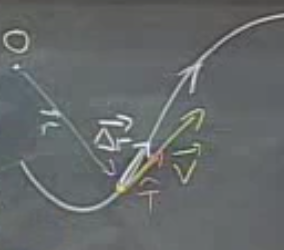
\includegraphics[height=4cm]{6_4.png}

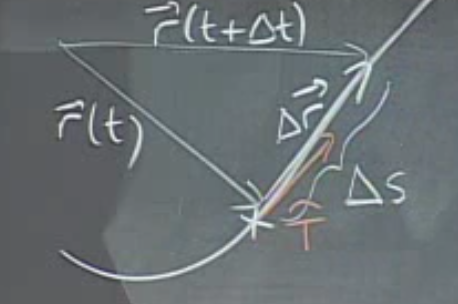
\includegraphics[height=4cm]{6_5.png}

Yerimizi $t$ aninda $\vec{r}(t)$, $\Delta t$ kadar bir adim atiyoruz, ve
$\vec{r}(t+\Delta t)$ noktasina geliyoruz. Bu noktada egri uzerinde
katedilen mesafe $\Delta s$, o zaman

\[ \frac{\Delta s}{\Delta t} \approx h�z \]

Yer vektorumuzun degisimi ise 

\[ \Delta \vec{r} \approx \hat{T} \Delta s \]

Iki tarafi $\Delta t$ ile bolersek 

\[ \frac{\Delta \vec{r}}{\Delta t} \approx \hat{T} \frac{\Delta s}{\Delta t} \]


ve $\Delta t \to 0$ olarak limitini alirsak, o zaman usttekiler turev
haline gelir, yaklasiksal isaret esitlik olur. Yani

\[ \frac{d\vec{r}}{dt} = \hat{T}\frac{ds}{dt} \]

Peki bu tur konularda vektorler kullanalim. Aslinda simdiye kadar
gorduklerimizi diger yollarla da temsil edebilirdik. Fakat vektor ``dili''
ozellikle hareketleri modellerken oldukca faydali oluyorlar. 

Ornek - Kepler'in Ikinci Kanunu

Kanun 1609'da kesfedildi, yani pek yeni bir gelisme oldugu iddia
edilemez. Kepler gezegenlerin hareketini modellemeye ugrasiyordu. Bazi
insanlar gezegenler mukemmel bir cember icinde donerler,
vs. diyordu. Kepler gezegenlerin yorungesinin cember degil elips (ellipse)
oldugunu one surdu. Kepler'in Kanunu soyle der:

Gezegenlerin hareketi bir duzlem uzerindedir, gunesten gezegene
cekilebilecek bir hayali cizginin kapsadigi alanin buyumesi / asilmasi
sabit bir orandadir. Bu ilginc bir kanun cunku bir kez yorungenin seklini
bilirsek, o yorunge uzerinde ne kadar hizli gidebilecegimizi bize
soyluyor. 

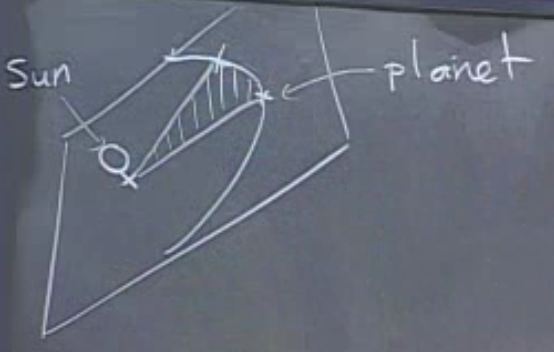
\includegraphics[height=4cm]{6_6.png}

Ustteki sekle bakarsak, gunes (sun) etrafinda bir gezegen (planet) var, ve
katedilen yol tarali sekilde cizili. Kepler Kanunu su anlama gelir,
katedilen alan zamana orantilidir, eger gezegen gunese daha yakin olsa,
daha hizli gitmek zorundadir, uzak olsa, daha yavas gitmek zorundadir, ki
katedilen alanin zamana orani ayni kalsin. Niye? Eger yakin olursak, gunese
direk mesafe azalacaktir, boydan kaybettigimizi diger yonden kazanmamiz
gerekir, yani ayni zamanda ayni alani katetmek icin bu sefer yorunde
uzerine daha hizli gidilmelidir, ki ayni alana erisebilelim. Tabii
gezegenlerin akli yoktur, boyle olsun diye ugrasmazlar, Kepler gozlemlerini
yaparken, modellerken degismeyen bu buyuklugu kesfetmistir, ve sayede bazi
hesaplari temiz sekilde yapabilmesi mumkun olmustur.

Biz de simdi bu kanunu, mekanik / fizikten bugun bildiklerimizi kullanarak
dogrulamaya calisacagiz. Newton, ki 1600'lu yillarin sonlarinda ortaya
cikti, bu durumu yercekimi formulleri ile aciklamayi basardi. 

Simdi vektorler kullanarak bu modeli yaratacagiz ve Kepler'in onlari
kullanarak alan hesabinin aslinda ne kadar dogal / bariz oldugunu
gorecegiz. Fakat Kepler bu kanunu ortaya atarken isler hicbir bu kadar
bariz degildi!

Tekrar bir pozisyon vektoru $\vec{r}$ yaratalim, baslangici gunes, bitis
noktasi gezegen olsun, katedilen yol $\Delta \vec{r}$ olsun. 

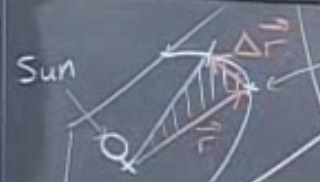
\includegraphics[height=3cm]{6_7.png}

Katedilen alani nasil hesaplariz. Sekilde cizdiklerimiz yeterince ipucu
veriyor, yaklasiksal olarak bir ucgen olustu. Alan bir kenari $\vec{r}$,
diger kenari $\Delta \vec{r}$ olan paralelogramin yarisi. Paralelogram
hesabini yapmayi biliyoruz nasilsa,

\[ 
\textrm{ $\Delta t$'de Kapsanan Alan } \approx
\frac{1}{2} |\vec{r} \times \Delta \vec{r}| 
\]

ki $\Delta t$ oldukca kucuk olmali. 

Ayrica

\[ \Delta \vec{r} \approx \vec{v} \Delta t \]

O zaman alan

\[ \approx
\frac{1}{2} |\vec{r} \times \vec{v}| \Delta t
 \]

Peki bu alanin zamana sabit oranda olmasi ne demektir? Alanin $\Delta t$'ye
oranli olmasi demektir, bu da ustteki formulde $|\vec{r} \times \vec{v}|$ teriminin 
sabit olmasi demektir. 

2. kanunu dusunelim, gezegenin yorungesinin hep ayni duzlem uzerinde
oldugunu soyluyordu. Bu demektir ki $\vec{r} \times \vec{v}$ ile ortaya
cikan ve bu ikisine normal (dik) olan ucuncu vektorun ``yonu'' hep ayni
kalmalidir. Cunku iki vektor bir duzlem tanimlar, bu iki vektore dik olan
duzleme de diktir, ve duzlem hic degismiyorsa bu vektorun yonu de
degisemez.

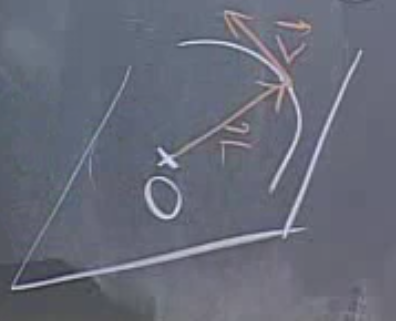
\includegraphics[height=4cm]{6_8.png}

O zaman hem buyukluk ayni, hem yon ayni, o zaman Kepler'in 2. Kanunu
$\vec{r} \times \vec{v}$ bir sabit vektor demektir. Ne yonu ne buyuklugu
degismeyecektir. 

Turevler baglaminda bunu soyle soyleyebiliriz

\[ \frac{d}{dt}(\vec{r} \times \vec{v}) = 0 \]

Turevler normal carpimlar icine nufuz ederken Carpim Kanunu (Product Rule)
kullaniliyordu. Capraz carpimlar icin de ayni kural gecerli, yani ustteki

\[ = \frac{\vec{r}}{dt} \times \vec{v} + \vec{r} \times \frac{d\vec{v}}{dt} \]

Daha once turettigimiz esitlikleri usttekilerin yerine koyarsak

\[ =\vec{v} \times \vec{v} + \vec{r} \times \vec{a} = 0\]

Bir vektorun kendisi ile capraz carpimi her zaman sifirdir. O zaman
$\vec{v} \times \vec{v} = 0$. Denklemden atilabilir. Geriye kalanlar

\[ = \vec{r} \times \vec{a} = 0\]

Ustteki ifade ne zaman dogru olabilir? Ya da genel olarak iki vektorun
capraz carpimi ne zaman sifirdir? Eger birbirlerine paraleller ise. Bu
demektir ki ivme $\vec{a}$ ile pozisyon $\vec{r}$ birbirine
paraleldir. Yani Kepler'in 2. Kanunu aslinda bunu soylemektedir. 

Ve biz bugun yercekim gucunun $\vec{r}$'e paralel oldugunu biliyoruz, yani
mesela gunesin bir gezegeni kendine direk bir yonde cektigini
biliyoruz. Demek ki ustteki ifadenin sifir oldugu da dogrudur. 

Not: Bu arada parallellik hem cekim, hem itme icin gecerli olurdu (her iki
durumda da yon paralel). Hakikaten elektriksel alanda parcaciklarin
cekilmesi ve itilmesi baglaminda da Kepler'in Kanunu aynen islemektedir. 

Soru

Diyelim ki $P$ noktasi bir kure (sphere) uzerinde hareket ediyor ve 

\[ OP = \vec{r}(t) = x(t)\hat{i} + y(t)\hat{j} + z(t)\hat{k}  \]

Hiz vektoru $\vec{v}$'nin her zaman pozisyon vektoru $\vec{r}$'ye dik
oldugunu $x,y,z$ kordinatlarini kullanmadan ve alttaki esitlikten 
faydalanarak

\begin{equation}\label{eq1}
\frac{d}{dt}\vec{a} \cdot \vec{b} =  
\frac{d\vec{a}}{dt} \cdot \vec{b} +
\vec{a} \cdot \frac{d\vec{b}}{dt} 
\end{equation}


ispatlayin. 

Cevap

Eger $\vec{r}$ ve $\vec{v}$ birbirine dik ise, o zaman $\vec{r} \cdot
\vec{v} = 0$ demektir. 

Bu arada hatirlayalim ki hiz pozisyon vektorunun zamana gore turevidir. 

\[ \vec{v} = \frac{d\vec{r}}{dt} \]

Suradan bir giris yapalim. Eger uzerinde olunan kurenin yaricapi $a$ ise, 

\[ \vec{r} \cdot \vec{r} = a^2 \]

Usttekinin formul \ref{eq1}'e gore turevini alalim

\[ 
\frac{d}{dt}\vec{r} \cdot \vec{r} =  
\frac{d\vec{r}}{dt} \cdot \vec{r} +
\vec{r} \cdot \frac{d\vec{r}}{dt} = 0
 \]

Sag taraf sifir cunku sabit $a^2$'nin turevi sifir. Buradaki onemli gozlem
sudur, esitligin sag tarafi ``$t$'ye bagli olmayan, sabit bir degerdir'', bunu
soyleyebiliyoruz, cunku problem bir kure uzerinde gezinildigi bize
soylemis. Bu onemli bir puf noktasi, bu bilgi sayesinde turevi alip sag tarafi
sifir yapabiliyoruz. Devam edelim

\[ 
2 \frac{d\vec{r}}{dt} \cdot \vec{r} = 0
\]

\[ \vec{v} \cdot \vec{r} = 0 \]

Demek ki iki vektor birbirine dik. 2 degeri formulden atildi, sag taraf
sifir oldugu icin onemli degil.

Soru

Bir onceki soruda ispatlananin tam ters yonunu ispatlayin. Eger $\vec{r}$
ve $\vec{v}$ dik ise, $P$'nin hareketi kesinlikle bir kure uzerinde olmak
zorundadir. 

Cevap

Biliyoruz ki

\[ \vec{r} \cdot \vec{r} = |r|^2 \]

Turevi alinca

\[ 
\frac{d}{dt}\vec{r} \cdot \vec{r} = 0 
 \]

Sag taraf sifir oldu cunku orada bir sabit vardi. Diger taraftan, eger
diklik oldugunu biliyorsak su dogru olmali

\[ \vec{v} \cdot \vec{r} = 0 \]

$\vec{v}$ ayni zamanda pozisyonun turevidir, ustte yerine koyalim

\[ 
\frac{d\vec{r}}{dt} \cdot \vec{r} = 0
\]

Onceden gormustuk ki 

\[ 
2 \frac{d\vec{r}}{dt} \cdot \vec{r} =
\frac{d}{dt}(\vec{r} \cdot \vec{r})   
 \]

Bu denklemin sol tarafi iki ustteki formulun sol tarafina benziyor, o zaman

\[ \frac{d}{dt}(\vec{r} \cdot \vec{r}) = 0 \]

Simdi sunu soralim: Turevi sifir olan sey nedir? Bir sabittir. 

\[ \vec{r} \cdot \vec{r} = c \textrm{ adinda bir sabit }\]

O zaman $|\vec{r}| = \sqrt{c}$. 

Eger $\vec{r}$'nin uzunlugu hic degismiyor ise, o zaman pozisyon bir kure
uzerinde hareket ediyor olmalidir.




\end{document}
